% !TeX program = xelatex
% !TeX encoding = UTF-8
% !TeX TXS-program:compile = txs:///xelatex | txs:///xelatex
\documentclass[aspectratio=169, table, 12pt]{beamer}

% Preamble bersama seluruh slide mata kuliah ini.
% Dipanggil dari slides/sessionXX/sessionXX.tex tepat sesudah baris
% \documentclass[aspectratio=169, table, 12pt]{beamer}
% Paket tambahan yang hanya dibutuhkan satu sesi ditulis di berkas sesi itu.

\usepackage{colortbl}
\usepackage{xcolor}
\usepackage{listings}
\usepackage{tabularx}
\usepackage{booktabs}
\usepackage{tikz}
\usepackage{pgfplots}
\usepackage{fontspec}
\usepackage[english,bahasai]{babel}
\pgfplotsset{compat=1.18}
\usetikzlibrary{arrows.meta, positioning, calc, fit, shapes.geometric,
  shapes.multipart, backgrounds, matrix, chains, trees}

\makeatletter
\def\input@path{{../theme/}}
\makeatother
\graphicspath{{../theme/}{../../figures/}}
% Stub symlink Windows memakai tema cadangan sampai aset institusi tersedia.
\IfFileExists{../theme/beamerthemePradita.sty}{%
  \usetheme{Pradita}
}{%
  \usetheme{Madrid}
  \setmainfont{TeX Gyre Heros}
  \setsansfont{TeX Gyre Heros}
  \setbeamertemplate{navigation symbols}{}
}

\definecolor{praditagreen}{RGB}{37, 113, 71}
\setbeamercolor{structure}{fg=praditagreen}
\setbeamercolor{palette primary}{bg=praditagreen,fg=white}
\setbeamercolor{palette secondary}{bg=praditagreen!80!black,fg=white}
\setbeamercolor{palette tertiary}{bg=praditagreen!60!black,fg=white}
\setbeamerfont{frametitle}{size=\large}
\setbeamertemplate{caption}[numbered]

% Ukuran header mengikuti teks agar judul panjang tidak menabrak logo.
\setbeamercolor{frametitle}{bg=white,fg=black}
\setbeamertemplate{frametitle}{%
  \begin{beamercolorbox}[wd=\paperwidth,sep=0.2cm]{frametitle}
    \begin{minipage}[c]{0.77\paperwidth}
      \raggedright\fontsize{16}{18}\selectfont\bfseries\insertframetitle
      \ifx\insertframesubtitle\empty\else
        \par\small\mdseries\insertframesubtitle
      \fi
    \end{minipage}\hfill
    \begin{minipage}[c]{0.15\paperwidth}
      \IfFileExists{../theme/classFiles/logo_universitas.png}{%
        
\includegraphics[width=\linewidth]{../theme/classFiles/logo_universitas.png}%
      }{}
    \end{minipage}
  \end{beamercolorbox}
}
\setbeamertemplate{footline}{%
  \ifnum\value{framenumber}>1
    \begin{beamercolorbox}[wd=\paperwidth,ht=0.35cm,dp=0.15cm,
      leftskip=0.3cm,rightskip=0.3cm]{palette primary}
      \footnotesize\bfseries\insertframenumber/\inserttotalframenumber
      \hfill IT40513
    \end{beamercolorbox}
  \fi
}
\DeclareRobustCommand{\berkas}[1]{\path{#1}}

% Tema membuat garis tabel berwarna putih. Dikembalikan agar tabel terbaca.
\arrayrulecolor{black}
\setlength{\arrayrulewidth}{0.5pt}

\lstdefinelanguage{yaml}{
  basicstyle=\ttfamily\scriptsize,
  keywordstyle=\color{blue}\bfseries,
  commentstyle=\color{gray}\itshape,
  stringstyle=\color{red},
  showstringspaces=false,
  breaklines=true,
  frame=lines,
  numbers=none,
  backgroundcolor=\color{lightgray!10},
  tabsize=2,
  morecomment=[l]{\#}
}

\lstdefinelanguage{json}{
  basicstyle=\ttfamily\scriptsize,
  stringstyle=\color{red},
  commentstyle=\color{gray},
  breaklines=true,
  showstringspaces=false,
  tabsize=2,
  numbers=none,
  frame=lines,
  backgroundcolor=\color{lightgray!10},
  string=[s]{"}{"}
}

\lstdefinelanguage{bash}{
  keywords={},
  basicstyle=\ttfamily\scriptsize,
  ndkeywords={docker, kubectl, helm, curl, git, terraform},
  ndkeywordstyle=\color{purple}\bfseries,
  sensitive=true,
  commentstyle=\color{gray},
  numbers=none,
  breaklines=true,
  frame=lines,
  backgroundcolor=\color{lightgray!10},
  tabsize=2,
  comment=[l]{\#},
  showstringspaces=false
}

\lstdefinelanguage{http}{
  keywords={GET, POST, PUT, PATCH, DELETE, HEAD, OPTIONS, HTTP},
  basicstyle=\ttfamily\scriptsize,
  keywordstyle=\color{blue}\bfseries,
  sensitive=true,
  numbers=none,
  breaklines=true,
  frame=lines,
  backgroundcolor=\color{lightgray!10},
  tabsize=2,
  showstringspaces=false
}

\subtitle{IT40513 · Enterprise Architecture \& Digital Blueprint}
\author{\textbf{Alfa Yohannis}}


% Sampul membatasi judul di panel putih tema rujukan Pradita.
\setbeamertemplate{title page}{%
  \begin{tikzpicture}[remember picture,overlay]
    \node[anchor=north west,inner sep=0pt,text width=8.8cm]
      at ([xshift=1cm,yshift=-3.15cm]current page.north west) {%
        {\small\insertsubtitle\par}\vspace{0.25cm}
        \resizebox{8.8cm}{!}{\begin{minipage}{12cm}
          \raggedright\color{praditagreen}\bfseries\inserttitle
        \end{minipage}}
      };
    \node[anchor=south west,inner sep=0pt]
      at ([xshift=1cm,yshift=1.65cm]current page.south west)
      {\small\insertdate};
    \node[anchor=west,inner sep=0pt,text=white]
      at ([xshift=0.8cm,yshift=0.75cm]current page.south west)
      {\small\insertauthor};
  \end{tikzpicture}
}


% Batasi kedua dimensi gambar agar diagram bersama tetap berada pada slide.
\newsavebox{\eafigbox}
\newcommand{\eadiagram}[1]{%
  \sbox{\eafigbox}{\resizebox{0.94\textwidth}{!}{\input{#1}}}%
  \ifdim\dimexpr\ht\eafigbox+\dp\eafigbox\relax>0.64\textheight
    \resizebox{!}{0.64\textheight}{\usebox{\eafigbox}}%
  \else
    \usebox{\eafigbox}%
  \fi
}


\newcolumntype{Y}{>{\raggedright\arraybackslash}X}
\newcolumntype{L}[1]{>{\raggedright\arraybackslash}p{#1}}

\title{\Huge Arsitektur Teknologi\\ \vspace{10pt} Target dan Kesiapan AI}
\date{Pertemuan 10}

\begin{document}

\frame{\titlepage}

\begin{frame}
  \frametitle{Isi Pertemuan}
  \vspace{14pt}
  \begin{columns}[t]
    \column{0.5\textwidth}
    {\small\tableofcontents[sections={1-3}]}

    \column{0.5\textwidth}
    {\small\tableofcontents[sections={4-5}]}
  \end{columns}
\end{frame}

\begin{frame}{\hfill}
  \centering
  \Huge{\textbf{Mengapa pilihan teknologi\\yang masuk akal per proyek\\berakhir mahal?}}
\end{frame}

\section{Tujuan dan Konteks}

\begin{frame}{\hfill}
  \centering
  \Huge{\textbf{Tujuan dan Konteks}}
\end{frame}

\begin{frame}{{\Large Tujuan Pembelajaran}}
  \vspace{10pt}
  \begin{itemize}
    \item Merumuskan arah teknologi target tingkat tinggi beserta standar teknologi organisasi.
    \item Mendokumentasikan keputusan arsitektur penting sebagai ADR (\textit{Architecture Decision
          Record}) lengkap dengan \textit{tradeoff}-nya.
    \item Menilai kesiapan organisasi memanfaatkan AI (\textit{Artificial Intelligence}) dari sisi
          kapabilitas, data, dan tata kelola.
  \end{itemize}
\end{frame}

\begin{frame}{{\Large Masalah: Keputusan Diambil per Proyek}}
  \small
  \vspace{6pt}
  \begin{itemize}
    \item Tiap proyek memilih teknologi sendiri, dan tiap pilihan masuk akal saat diambil.
    \item Lima tahun kemudian ada empat merek basis data, enam alat pelaporan, dan dua cara menyimpan
          cadangan.
    \item Biayanya muncul di tiga tempat: lisensi tumpang tindih, keahlian tersebar tipis, dan celah
          keamanan.
    \item Fase D ADM (\textit{Architecture Development Method}) menutup rancangan kondisi target.
  \end{itemize}
  \vspace{6pt}
  Empat pertanyaan bab ini: layanan teknologi apa, dijalankan di mana, standar apa yang mengikat
  proyek berikutnya, dan bagaimana keputusan besar dicatat.
\end{frame}

\begin{frame}{{\Large Diagram Konsep Bab 10}}
  \centering
  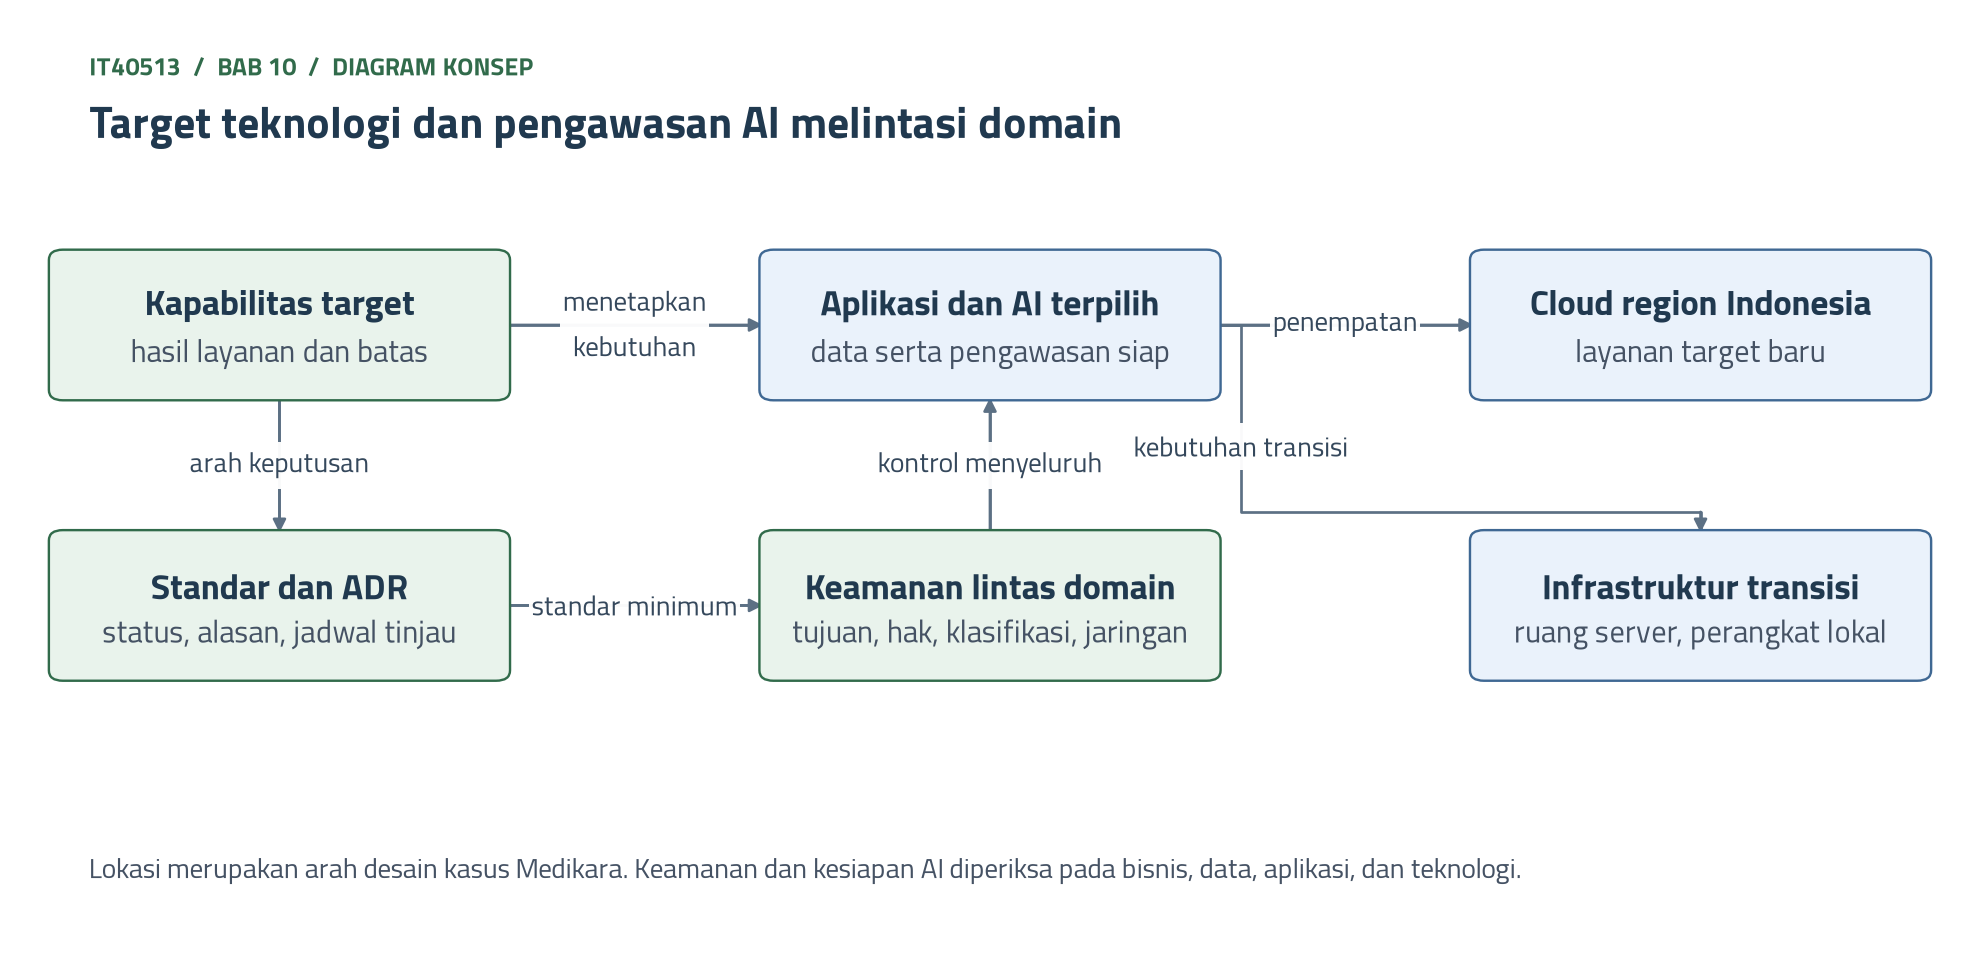
\includegraphics[width=0.96\textwidth,height=0.77\textheight,keepaspectratio]{../../figures/ch10-diagram-konsep.png}
  \label{fig:session10-ilustrasi-bab}
\end{frame}

\section{Arah, Standar, dan Keamanan}

\begin{frame}{\hfill}
  \centering
  \Huge{\textbf{Arah, Standar,\\dan Keamanan}}
\end{frame}

\begin{frame}{{\Large Arsitektur Teknologi Tingkat Tinggi}}
  \small
  \vspace{6pt}
  \begin{itemize}
    \item Menjelaskan layanan teknologi yang dibutuhkan aplikasi dan data target, beserta tempat
          layanan itu dijalankan.
    \item Yang diputuskan adalah arah, bukan ukuran server atau versi pustaka perangkat lunak.
    \item Rincian di bawah arah itu menjadi urusan arsitektur solusi tiap proyek.
    \item Lima tim dengan lima jenis basis data diganti satu layanan terkelola dengan dua pilihan
          standar.
  \end{itemize}
  \vspace{6pt}
  Analogi: utilitas gedung. Penyewa membutuhkan jaminan listrik, air, lift, dan pengamanan pintu yang
  sama di setiap lantai.
\end{frame}

\begin{frame}{{\Large Arah Teknologi Target Medikara}}
  \centering
  \begin{figure}
    \resizebox{0.86\textwidth}{!}{\begin{tikzpicture}[
  font=\scriptsize,
  kotak/.style={draw, rounded corners, minimum height=0.85cm, text width=1.6cm,
                align=center, font=\scriptsize},
  lokasi/.style={draw, rounded corners, minimum height=0.85cm, text width=2.6cm,
                 align=center, font=\scriptsize},
  pita/.style={draw, rounded corners, fill=praditagreen!15, minimum height=1.2cm,
               text width=1.6cm, align=center, font=\scriptsize\bfseries},
  panah/.style={-{Stealth[length=2mm]}, thick}
]
  % Pita kiri: tiga lapis pertanyaan arsitektur teknologi.
  \node[pita] (p1) at (0,3.4) {Aplikasi\\target};
  \node[pita] (p2) at (0,1.7) {Layanan\\teknologi};
  \node[pita] (p3) at (0,0) {Lokasi\\penerapan};

  % Lapis atas: aplikasi target dari Bab 9.
  \node[kotak, fill=blue!8] at (2.2,3.4) {SIMRS\\terpadu};
  \node[kotak, fill=blue!8] at (4.15,3.4) {MPI};
  \node[kotak, fill=blue!8] at (6.1,3.4) {Platform\\integrasi};
  \node[kotak, fill=blue!8] at (8.05,3.4) {Medikara+,\\portal mitra};
  \node[kotak, fill=blue!8] at (10.0,3.4) {ERP dan\\platform data};

  % Lapis tengah: layanan teknologi yang dirumuskan di fase D.
  \node[kotak, fill=orange!12] at (2.2,1.7) {Basis data\\terkelola};
  \node[kotak, fill=orange!12] at (4.15,1.7) {Identitas\\terpusat};
  \node[kotak, fill=orange!12] at (6.1,1.7) {Integrasi dan\\\textit{API gateway}};
  \node[kotak, fill=orange!12] at (8.05,1.7) {Penyim\-panan,\\cadangan};
  \node[kotak, fill=orange!12] at (10.0,1.7) {Pemantauan,\\catatan akses};

  % Lapis bawah: lokasi penerapan.
  \node[lokasi, fill=green!10] at (3.0,0) {\textit{Cloud} publik region\\Indonesia {\tiny\mdseries(arah utama)}};
  \node[lokasi, fill=blue!8] at (6.1,0) {Ruang server rumah sakit\\{\tiny\mdseries(selama transisi)}};
  \node[lokasi, fill=blue!8] at (9.2,0) {Rumah sakit dan klinik\\{\tiny\mdseries(jaringan, perangkat lokal)}};

  \draw[panah] (p1.south) -- (p2.north);
  \draw[panah] (p2.south) -- (p3.north);
  \node[font=\tiny, gray, anchor=west] at (0.1,2.55) {membutuhkan};
  \node[font=\tiny, gray, anchor=west] at (0.1,0.85) {dijalankan di};
\end{tikzpicture}
}
    \caption{Aplikasi target membutuhkan layanan teknologi bersama, dan layanan itu dijalankan di
             lokasi yang ditetapkan}
  \end{figure}
\end{frame}

\begin{frame}{{\Large Empat Pilihan Lokasi Penerapan}}
  \scriptsize
  \begin{tabularx}{\textwidth}{L{1.7cm}YYY}
    \hline
    \textbf{Pilihan} & \textbf{Artinya} & \textbf{Cocok untuk} & \textbf{Yang dikorbankan} \\
    \hline
    \textit{On-premise} & Server milik dan dikelola sendiri di lokasi sendiri &
      Sistem yang terikat perangkat lokal atau kontrak lama &
      Modal awal besar, kapasitas tetap, pemulihan bencana ditanggung sendiri \\
    \hline
    \textit{Private cloud} & Infrastruktur \textit{cloud} khusus untuk satu organisasi &
      Organisasi besar yang butuh kendali penuh dan elastisitas &
      Tetap butuh tim dan skala besar agar efisien \\
    \hline
    \textit{Public cloud} & Infrastruktur penyedia yang dipakai banyak pelanggan, dibayar sesuai pemakaian &
      Beban yang naik turun, layanan baru, analitik &
      Ketergantungan pada penyedia, biaya berulang yang harus dikendalikan \\
    \hline
    \textit{Hybrid cloud} & Dua model atau lebih yang terpisah tetapi terhubung &
      Masa transisi, beban yang belum dapat dipindahkan &
      Dua lingkungan yang harus dikelola dan diamankan sekaligus \\
    \hline
  \end{tabularx}
\end{frame}

\begin{frame}{{\Large Lokasi Rekam Medis Dibatasi Regulasi}}
  \small
  \vspace{6pt}
  \begin{itemize}
    \item EA (\textit{Enterprise Architecture}) menetapkan arah dan aturan pemilihan, misalnya
          \textit{cloud} publik di region Indonesia untuk aplikasi baru.
    \item Permenkes 24/2022 Pasal 20: server, komputasi awan tersertifikasi, atau media digital lain
          yang tersertifikasi.
    \item Cadangan wajib berada di tempat berbeda dari fasilitas. Medikara punya 23 fasilitas yang
          terkena kewajiban ini.
    \item Pasal 22: Penyelenggara Sistem Elektronik harus punya fasilitas penyimpanan di dalam negeri
          dan rekomendasi Kementerian Kesehatan.
    \item Strategi 7R dan \textit{landing zone} dibahas rinci di IT40713.
  \end{itemize}
\end{frame}

\begin{frame}{{\Large Arah Modernisasi ke Cloud dan Batasannya}}
  \begin{block}{Kasus Medikara Health}
    \small
    \begin{itemize}
      \item \textit{Cloud} publik di region Indonesia untuk SIMRS (Sistem Informasi Manajemen Rumah
            Sakit) terpadu, MPI (\textit{Master Patient Index}), platform integrasi, dan platform data.
      \item Ruang server tiap rumah sakit dipakai selama transisi, lalu ditutup bertahap.
      \item Rumah sakit dan klinik hanya menyimpan perangkat yang harus dekat dengan pasien.
    \end{itemize}
    \vspace{4pt}
    Empat batasan: regulasi rekam medis, jaringan (misalkan dua klinik Bogor hanya punya satu jalur
    internet), keterampilan tim, dan kontrak vendor SIMRS lama.
  \end{block}
\end{frame}

\begin{frame}{{\Large Katalog Standar Teknologi}}
  \small Katalog berisi teknologi yang disepakati beserta versi, status, pemilik, dan jadwal peninjauan.
  Analogi: formularium rumah sakit. Technology Radar hanya pendapat satu perusahaan, katalog mengikat
  proyek sendiri.

  \centering
  \begin{figure}
    \resizebox{0.84\textwidth}{!}{\begin{tikzpicture}[
  font=\scriptsize,
  kotak/.style={draw, rounded corners, minimum height=1.05cm, text width=1.7cm,
                align=center, font=\scriptsize\bfseries},
  panah/.style={-{Stealth[length=2mm]}, thick}
]
  \node[kotak, fill=blue!8] (usul) at (0,0) {Usulan\\{\tiny\mdseries diajukan proyek}};
  \node[kotak, fill=blue!8] (baru) at (2.5,0) {Baru\\{\tiny\mdseries uji coba terbatas}};
  \node[kotak, fill=green!10] (pakai) at (5.0,0) {Dipakai\\{\tiny\mdseries wajib untuk proyek baru}};
  \node[kotak, fill=orange!12] (batas) at (7.5,0) {Dibatasi\\{\tiny\mdseries hanya dipelihara}};
  \node[kotak, fill=red!22] (henti) at (10.0,0) {Dihentikan\\{\tiny\mdseries tanggal akhir pasti}};
  \node[kotak, fill=gray!35] (tolak) at (2.5,-1.85) {Ditolak\\{\tiny\mdseries alasan dicatat}};

  \draw[panah] (usul) -- (baru);
  \draw[panah] (baru) -- (pakai);
  \draw[panah] (pakai) -- (batas);
  \draw[panah] (batas) -- (henti);
  \draw[panah] (baru) -- (tolak);

  \node[font=\tiny, gray] at (1.25,0.78) {disetujui dicoba};
  \node[font=\tiny, gray] at (3.75,0.78) {lolos uji coba};
  \node[font=\tiny, gray] at (6.25,0.78) {ada pengganti};
  \node[font=\tiny, gray] at (8.75,0.78) {migrasi selesai};
  \node[font=\tiny, gray, anchor=west] at (2.6,-0.95) {gagal uji coba};

  \node[font=\tiny, align=center, text width=6.2cm, anchor=north west]
    at (4.15,-1.3) {Setiap perpindahan status diputuskan forum arsitektur,
    dicatat sebagai ADR, dan ditinjau ulang paling lambat 12 bulan sekali.};
\end{tikzpicture}
}
    \caption{Setiap teknologi masuk lewat uji coba dan keluar lewat tanggal akhir yang pasti}
  \end{figure}
\end{frame}

\begin{frame}{{\Large Potongan Katalog Standar Medikara}}
  \scriptsize
  \begin{tabularx}{\textwidth}{Yl Y}
    \hline
    \textbf{Standar} & \textbf{Status} & \textbf{Catatan} \\
    \hline
    Basis data relasional sumber terbuka sebagai layanan terkelola & Dipakai & Pilihan pertama untuk aplikasi baru \\
    \hline
    Basis data relasional komersial bawaan SIMRS lama & Dibatasi & Hanya dipelihara sampai SIMRS diganti \\
    \hline
    Sistem operasi server versi lama tanpa dukungan vendor & Dihentikan & Tanggal akhir 31 Desember 2027 \\
    \hline
    Layanan identitas terpusat dengan autentikasi multifaktor & Dipakai & Wajib untuk semua aplikasi baru \\
    \hline
    HL7 (\textit{Health Level Seven}) FHIR (\textit{Fast Healthcare Interoperability Resources}) untuk data klinis & Dipakai & Sejalan dengan SATUSEHAT \\
    \hline
    Platform analitik dan \textit{dashboard} tunggal & Baru & Uji coba di rumah sakit Depok sampai Juni 2027 \\
    \hline
    \textit{Spreadsheet} sebagai sumber laporan manajemen & Dibatasi & Diganti platform analitik \\
    \hline
  \end{tabularx}
\end{frame}

\begin{frame}{{\Large Dua Konsekuensi Standardisasi}}
  \small
  \vspace{6pt}
  \begin{itemize}
    \item Biaya rutin turun: misalkan lisensi dan dukungan empat merek basis data Rp2,4 miliar per
          tahun menjadi Rp1,5 miliar untuk dua merek.
    \item Penghematannya Rp0,9 miliar per tahun.
    \item Keahlian terpusat: dengan dua administrator per merek, delapan orang menjadi empat orang.
    \item Biaya di depan: migrasi satu kali Rp2,7 miliar baru tertutup dalam tiga tahun.
    \item Biaya tersembunyi: ketergantungan pada vendor yang lebih sedikit makin besar, dan proyek
          terhambat bila jalur status Baru tidak tersedia.
  \end{itemize}
\end{frame}

\begin{frame}{{\Large Technology Reference Model}}
  \small
  \vspace{6pt}
  \begin{itemize}
    \item Taksonomi layanan platform generik: manajemen data, keamanan, jaringan, antarmuka pengguna.
    \item TOGAF \textit{Technical Reference Model} kini tersedia sebagai \textit{Series Guide} G175:
          konten historis yang masih berguna.
    \item Nilai utamanya bahasa bersama. ``Sistem laporan'', ``platform analitik'', dan
          \textit{business intelligence} merujuk kategori yang sama.
    \item \textit{Technology reference model} adalah rak berlabel. Katalog standar adalah isi rak.
    \item Organisasi boleh meminjam rak dari luar, tetapi isi rak diputuskan sendiri.
  \end{itemize}
\end{frame}

\begin{frame}{{\Large Keamanan sebagai Concern Lintas Domain}}
  \footnotesize
  \begin{tabularx}{\textwidth}{L{1.7cm}YY}
    \hline
    \textbf{Domain} & \textbf{Pertanyaan keamanan} & \textbf{Contoh keputusan arsitektur} \\
    \hline
    Bisnis & Peran apa yang boleh melihat rekam medis? & Hanya tenaga kesehatan yang merawat pasien itu \\
    \hline
    Data & Data mana yang paling dilindungi? & Data kesehatan diklasifikasi sebagai data pribadi spesifik \\
    \hline
    Aplikasi & Di mana hak akses diperiksa? & Semua aplikasi memakai satu layanan identitas dan peran baku \\
    \hline
    Teknologi & Dari mana basis data klinis dapat dijangkau? & Hanya dari zona aplikasi, tidak dari jaringan umum \\
    \hline
  \end{tabularx}

  \vspace{6pt}
  \small UU 27/2022 tentang Pelindungan Data Pribadi (PDP) menggolongkan data kesehatan sebagai data
  pribadi yang bersifat spesifik. Kewajibannya dibahas rinci di IT40813.
\end{frame}

\begin{frame}{{\Large Tiga Keputusan Keamanan Terpenting}}
  \small
  \vspace{6pt}
  \begin{itemize}
    \item Identitas terpusat: satu akun untuk semua sistem, termasuk dokter mitra dan teknisi vendor.
    \item Kontrol akses berbasis peran dengan hak minimum.
    \item Pemisahan jaringan menjadi zona: pembobolan satu zona tidak langsung membuka zona lain.
    \item Ketiganya sejalan dengan \textit{zero trust} dan diambil sejak rancangan (\textit{security by
          design}).
    \item Misalkan akun di tujuh sistem. Bila 8 persen dari 4.800 karyawan keluar, 384 orang berarti
          2.688 pencabutan manual, atau 384 pencabutan bila terpusat.
  \end{itemize}
\end{frame}

\begin{frame}{{\Large Zona Keamanan Target}}
  \centering
  \begin{figure}
    \resizebox{0.80\textwidth}{!}{\begin{tikzpicture}[
  font=\scriptsize,
  aktor/.style={draw, rounded corners, fill=blue!8, minimum height=0.8cm,
                text width=1.8cm, align=center, font=\scriptsize},
  kotak/.style={draw, rounded corners, minimum height=1.2cm, text width=2.0cm,
                align=center, font=\scriptsize\bfseries},
  zona/.style={draw, rounded corners, minimum height=0.8cm, text width=2.7cm,
               align=center, font=\scriptsize},
  panah/.style={-{Stealth[length=2mm]}, thick}
]
  % Kiri: siapa yang meminta akses.
  \node[aktor] (pasien) at (0,2.4) {Pasien};
  \node[aktor] (staf) at (0,1.2) {Karyawan\\dan dokter};
  \node[aktor] (vendor) at (0,0) {Vendor\\dan mitra};

  % Tengah: satu pintu identitas, lalu satu pengatur hak.
  \node[kotak, fill=praditagreen!15] (idp) at (3.0,1.2)
    {Identitas terpusat\\{\tiny\mdseries satu akun per orang,\\autentikasi multifaktor}};
  \node[kotak, fill=orange!12] (hak) at (5.9,1.2)
    {Kontrol akses\\{\tiny\mdseries hak minimum\\sesuai peran}};

  % Kanan: zona yang dipisahkan.
  \node[zona, fill=blue!8] (publik) at (9.4,2.4) {Zona publik\\{\tiny Medikara+, portal mitra}};
  \node[zona, fill=blue!8] (apl) at (9.4,1.2) {Zona aplikasi\\{\tiny SIMRS, ERP, integrasi}};
  \node[zona, fill=orange!12] (klinis) at (9.4,0) {Zona data klinis\\{\tiny rekam medis, MPI}};

  % Bawah: bukti dan kondisi lama sebagai pembanding.
  \node[zona, fill=green!10] (log) at (5.9,-1.65) {Catatan akses terpusat\\{\tiny siapa, kapan, data apa}};
  \node[zona, fill=red!22] (lama) at (0.4,-1.65) {Kondisi 2025\\{\tiny akun vendor bersama,\\jaringan datar}};

  \draw[panah] (pasien.east) -- (idp.west);
  \draw[panah] (staf.east) -- (idp.west);
  \draw[panah] (vendor.east) -- (idp.west);
  \draw[panah] (idp) -- (hak);
  \draw[panah] (hak.east) -- (publik.west);
  \draw[panah] (hak.east) -- (apl.west);
  \draw[panah] (hak.east) -- (klinis.west);
  \draw[panah, dashed, gray] (klinis.south) |- (log.east);
  \draw[panah, dashed, gray] (idp.south) |- (log.west);

  \node[font=\tiny, gray, anchor=north west, text width=2.6cm, align=left]
    at (-0.95,-0.45) {target: akun vendor pribadi\\dan berbatas waktu};
\end{tikzpicture}
}
    \caption{Satu pintu identitas, satu pengatur hak, dan zona yang dipisahkan. Kotak merah adalah
             kondisi 2025 yang diganti}
  \end{figure}
\end{frame}

\begin{frame}{{\Large Audit Kontrol Akses dan Insiden Vendor}}
  \begin{block}{Kasus Medikara Health}
    \small
    Misalkan penelusuran menemukan empat hal: akun vendor dipakai bersama dengan satu kata sandi, akun
    aktif terus-menerus, jaringan rumah sakit datar, dan 212 akun aktif milik orang yang sudah keluar.
    \vspace{2pt}
    \begin{itemize}
      \item Satu layanan identitas dengan autentikasi multifaktor.
      \item Peran baku di semua aplikasi, sehingga pencabutan cukup sekali.
      \item Zona data klinis hanya dari zona aplikasi. Akses vendor per permintaan.
      \item Catatan akses terpusat: siapa membuka data apa dan kapan.
    \end{itemize}
  \end{block}
\end{frame}

\section{Keputusan Arsitektur dan ADR}

\begin{frame}{\hfill}
  \centering
  \Huge{\textbf{Keputusan Arsitektur\\dan ADR}}
\end{frame}

\begin{frame}{{\Large Struktur ADR}}
  \small ADR mencatat satu keputusan penting beserta alasannya. Keputusan yang dibatalkan ditandai
  digantikan, tidak dihapus.

  \vspace{4pt}
  \footnotesize
  \begin{tabularx}{\textwidth}{L{2.5cm}YL{4.0cm}}
    \hline
    \textbf{Bagian} & \textbf{Isinya} & \textbf{Pertanyaan yang dijawab} \\
    \hline
    Nomor dan judul & ADR-001, frasa benda singkat & Keputusan tentang apa? \\
    \hline
    Status & Diusulkan, diterima, atau digantikan oleh ADR lain & Masih berlaku atau tidak? \\
    \hline
    Konteks & Masalah, batasan, asumsi, prinsip yang terkait & Mengapa harus diputuskan sekarang? \\
    \hline
    Opsi dan kriteria & Minimal dua opsi, kriteria berbobot yang ditetapkan lebih dahulu & Apa saja yang dipertimbangkan? \\
    \hline
    Keputusan & Satu kalimat aktif beserta syaratnya & Apa yang dipilih? \\
    \hline
    Konsekuensi & Dampak positif, negatif, dan pekerjaan lanjutan & Apa harga pilihan ini? \\
    \hline
  \end{tabularx}
\end{frame}

\begin{frame}{{\Large Penilaian Tiga Opsi Lokasi Rekam Medis}}
  \small A: pusat data sendiri. B: \textit{cloud} publik tersertifikasi region Indonesia. C:
  \textit{hybrid}. Skor 1 sampai 5.

  \vspace{4pt}
  \footnotesize
  \begin{tabularx}{\textwidth}{Xrrrr}
    \hline
    \textbf{Kriteria} & \textbf{Bobot} & \textbf{A} & \textbf{B} & \textbf{C} \\
    \hline
    Kepatuhan regulasi dan lokasi data & 30\% & 5 & 4 & 4 \\
    \hline
    Keamanan dan kendali akses & 20\% & 3 & 4 & 3 \\
    \hline
    Ketersediaan dan pemulihan bencana & 20\% & 2 & 5 & 4 \\
    \hline
    Biaya lima tahun & 15\% & 2 & 4 & 3 \\
    \hline
    Keterampilan tim dan ketergantungan vendor & 15\% & 3 & 3 & 2 \\
    \hline
    \textbf{Skor berbobot} & 100\% & \textbf{3,25} & \textbf{4,05} & \textbf{3,35} \\
    \hline
  \end{tabularx}

  \vspace{4pt}
  \small Bobot ditetapkan sebelum opsi dinilai. Selisih 0,8 antara B dan A sebagian besar berasal dari
  kriteria ketersediaan.
\end{frame}

\begin{frame}{{\Large Kapan Keputusan Layak Dicatat}}
  \small
  \vspace{6pt}
  \begin{itemize}
    \item Mahal atau lama untuk dibatalkan, misalnya lokasi data dan platform inti.
    \item Berdampak pada lebih dari satu tim atau domain, misalnya pola integrasi.
    \item Menyimpang dari standar atau prinsip arsitektur.
    \item Menyentuh kepatuhan atau keselamatan pasien.
  \end{itemize}
  \vspace{6pt}
  ADR mencatat satu keputusan dan alasannya. Dokumen rancangan menjelaskan cara membangun dan berubah
  mengikuti pekerjaan. ADR yang sudah diterima tidak diubah isinya.

  \vspace{6pt}
  Analogi: notulen rapat RT yang mencatat alasan, opsi yang ditolak, dan pihak yang menanggung akibat.
\end{frame}

\begin{frame}{{\Large ADR-001 Lokasi Rekam Medis Elektronik}}
  \begin{block}{Kasus Medikara Health}
    \footnotesize
    \textbf{Status.} Diusulkan untuk forum arsitektur, Oktober 2026.

    \textbf{Konteks.} 5 rumah sakit dan 18 klinik disatukan ke SIMRS terpadu dan MPI. Pasal 20 dan 22
    Permenkes 24/2022 mengikat. Ruang server RS Jakarta tidak punya lokasi cadangan.

    \textbf{Keputusan.} Opsi B, dengan tiga syarat: sertifikasi penyedia diperiksa sebelum kontrak,
    cadangan di zona lain di dalam negeri, kunci enkripsi dikelola Medikara.

    \textbf{Konsekuensi.} Positif: pusat data sendiri tidak perlu dibangun. Negatif: ketergantungan pada
    satu penyedia, biaya bulanan, dan pelatihan \textit{cloud} bagi tim TI.
  \end{block}
\end{frame}

\section{AI dan Tata Kelola AI}

\begin{frame}{\hfill}
  \centering
  \Huge{\textbf{AI dan Tata Kelola AI}}
\end{frame}

\begin{frame}{{\Large AI sebagai Kapabilitas dan Concern}}
  \small
  \vspace{4pt}
  \begin{itemize}
    \item Urutan: kapabilitas, \textit{value stream}, ukuran keberhasilan, data, aplikasi dan teknologi,
          tata kelola. Produk dipilih paling akhir.
    \item Gartner: 63 persen organisasi tidak punya, atau tidak yakin punya, praktik data yang tepat
          untuk AI.
    \item Gartner memperkirakan sampai 2026 organisasi meninggalkan 60 persen proyek AI tanpa data yang
          siap.
    \item Kesiapan data: ketersediaan, mutu, identitas, dasar hukum, dan asal-usul.
    \item Model AI memberi keluaran. Agen AI juga bertindak, sehingga butuh identitas, hak terbatas,
          pemilik, dan catatan kegiatan.
  \end{itemize}
\end{frame}

\begin{frame}{{\Large Tahap Kematangan AI Enterprise}}
  \footnotesize
  \begin{tabularx}{\textwidth}{Xrrr}
    \hline
    \textbf{Tahap} & \textbf{Perusahaan} & \textbf{Pertumbuhan} & \textbf{Laba} \\
    \hline
    1. \textit{Experiment and Prepare} & 28\% & $-12{,}6$ & $-9{,}6$ \\
    \hline
    2. \textit{Build Pilots and Capabilities} & 34\% & $-3{,}5$ & $-2{,}2$ \\
    \hline
    3. \textit{Develop AI Ways of Working} & 31\% & $+11{,}3$ & $+8{,}7$ \\
    \hline
    4. \textit{Become AI Future Ready} & 7\% & $+17{,}1$ & $+10{,}4$ \\
    \hline
  \end{tabularx}

  \vspace{6pt}
  \small
  \begin{itemize}
    \item Survei MIT CISR terhadap 721 perusahaan. Kinerja dalam poin persentase terhadap rata-rata
          industri.
    \item Sebanyak 62 persen perusahaan masih di tahap 1 dan 2.
    \item Tabel ini menunjukkan keterkaitan, bukan sebab akibat.
  \end{itemize}
\end{frame}

\begin{frame}{{\Large Empat Model Operasi TI di Era AI}}
  \centering
  \begin{figure}
    \resizebox{0.66\textwidth}{!}{\begin{tikzpicture}[
  font=\scriptsize,
  sel/.style={draw, minimum width=4.4cm, minimum height=2.15cm, align=center,
              font=\scriptsize},
  tanda/.style={draw, rounded corners, minimum height=0.5cm, align=center,
                font=\tiny\bfseries},
  panah/.style={-{Stealth[length=2mm]}, thick}
]
  % Empat sel model operasi TI menurut MIT CISR.
  \node[sel, fill=gray!35] (lm) at (0,0)
    {\textbf{Legacy Modernizer}\\33\% perusahaan\\{\tiny\mdseries 37\% pendapatan dari inovasi}};
  \node[sel, fill=blue!8] (cs) at (0,2.15)
    {\textbf{Creative Sprinter}\\16\% perusahaan\\{\tiny\mdseries 49\% pendapatan dari inovasi}};
  \node[sel, fill=green!10] (ai) at (4.4,2.15)
    {\textbf{Adaptive Innovator}\\33\% perusahaan\\{\tiny\mdseries 71\% pendapatan dari inovasi}};
  \node[sel, fill=orange!12] (eb) at (4.4,0)
    {\textbf{Efficient Builder}\\18\% perusahaan\\{\tiny\mdseries 54\% pendapatan dari inovasi}};

  % Sumbu.
  \draw[panah] (-2.2,-1.25) -- (6.8,-1.25);
  \draw[panah] (-2.4,-1.07) -- (-2.4,3.4);
  \node[font=\tiny, anchor=north, align=center] at (2.2,-1.35)
    {kepemimpinan TI \textit{enterprise}, modularitas, dan pemakaian ulang (rendah ke tinggi)};
  \node[font=\tiny, rotate=90, anchor=south] at (-2.5,1.07)
    {kecepatan inovasi (rendah ke tinggi)};

  % Posisi Medikara menurut tafsiran bab ini.
  \node[tanda, fill=red!22] (kini) at (-0.9,-0.8) {Medikara kini};
  \node[tanda, fill=green!10] (arah) at (3.4,-0.8) {arah target};
  \draw[panah, red!65!black] (kini) -- (arah);
\end{tikzpicture}
}
    \caption{Empat model operasi TI di era AI menurut MIT CISR, dengan posisi Medikara menurut
             tafsiran bab ini}
  \end{figure}
\end{frame}

\begin{frame}{{\Large Dua Peluang AI}}
  \begin{block}{Kasus Medikara Health}
    \scriptsize
    \begin{tabularx}{\linewidth}{L{2.6cm}YY}
      \hline
      \textbf{Aspek} & \textbf{Prediksi antrean} & \textbf{Ringkasan rekam medis} \\
      \hline
      Kapabilitas & Pengelolaan kapasitas layanan & Pengelolaan rekam medis \\
      \hline
      Ukuran keberhasilan & Waktu tunggu rawat jalan turun 20\% & Waktu dokter membaca riwayat turun separuh \\
      \hline
      Kesiapan kapabilitas & 2: manajer rawat jalan siap memakai prediksi & 2: dokter mau mencoba, alur persetujuan belum ada \\
      \hline
      Kesiapan data & 2: dua dari lima SIMRS tidak mencatat waktu dipanggil & 1: identitas pasien ganda, MPI belum berjalan \\
      \hline
      Kesiapan tata kelola & 3: tidak menyentuh keputusan klinis & 1: data kesehatan, kebijakan AI belum ada \\
      \hline
      Syarat mulai & Pencatatan waktu diseragamkan & MPI dari Bab 9 dan kebijakan AI dari IT40813 \\
      \hline
    \end{tabularx}

    \vspace{4pt}
    \footnotesize Prediksi antrean dapat dimulai sebagai uji coba di satu rumah sakit pada 2027.
    Ringkasan rekam medis menunggu MPI dan kebijakan AI.
  \end{block}
\end{frame}

\begin{frame}{{\Large Pendalaman: Lima Titik Kendali}}
  \centering
  \begin{figure}
    \resizebox{0.88\textwidth}{!}{\begin{tikzpicture}[
  font=\scriptsize,
  kotak/.style={draw, rounded corners, minimum height=1.1cm, text width=1.65cm,
                align=center, font=\scriptsize\bfseries},
  kendali/.style={circle, draw, fill=red!22, inner sep=1pt, font=\tiny\bfseries},
  panah/.style={-{Stealth[length=2mm]}, thick}
]
  \node[kotak, fill=blue!8] (sumber) at (0,0)
    {Sumber data\\{\tiny\mdseries SIMRS, laboratorium, MPI}};
  \node[kotak, fill=blue!8] (pipa) at (2.45,0)
    {Pipeline data\\{\tiny\mdseries ekstraksi, format FHIR}};
  \node[kotak, fill=orange!12] (model) at (4.9,0)
    {Model ringkasan\\{\tiny\mdseries layanan model bahasa}};
  \node[kotak, fill=blue!8] (ui) at (7.35,0)
    {Antarmuka dokter\\{\tiny\mdseries draf di layar SIMRS}};
  \node[kotak, fill=green!10] (rm) at (9.8,0)
    {Rekam medis\\{\tiny\mdseries setelah disetujui dokter}};
  \node[kotak, fill=praditagreen!15, text width=4.2cm] (pantau) at (6.1,-2.0)
    {Pemantauan\\{\tiny\mdseries mutu ringkasan, keluhan dokter, catatan akses}};

  \draw[panah] (sumber) -- (pipa);
  \draw[panah] (pipa) -- (model);
  \draw[panah] (model) -- (ui);
  \draw[panah] (ui) -- (rm);
  \draw[panah, dashed, gray] (model.south) -- (model.south |- pantau.north);
  \draw[panah, dashed, gray] (ui.south) -- (ui.south |- pantau.north);
  \draw[panah, dashed, gray] (pantau.west) -| (pipa.south);

  % Titik kendali K1 sampai K5.
  \node[kendali] at (1.225,0.32) {K1};
  \node[kendali] at (3.675,0.32) {K2};
  \node[kendali] at (4.9,0.8) {K3};
  \node[kendali] at (8.575,0.32) {K4};
  \node[kendali] at (8.45,-2.0) {K5};
  \node[font=\tiny, gray, anchor=north] at (3.0,-2.1) {umpan balik perbaikan};
\end{tikzpicture}
}
    \caption{Komponen teknis ringkasan rekam medis dan lima titik kendalinya}
  \end{figure}
  \vspace{-4pt}
  \small Hanya K3 yang menyangkut model. Empat lainnya menyangkut data, alur kerja, dan pemantauan,
  yaitu wilayah yang sudah dikenal arsitek.
\end{frame}

\begin{frame}{{\Large Celah Visibilitas Agen AI}}
  \footnotesize
  \begin{tabularx}{\textwidth}{Xr}
    \hline
    \textbf{Temuan SAP LeanIX Agentic AI Survey 2026} & \textbf{Angka} \\
    \hline
    Sudah memakai agen AI (44\%), bereksperimen (40\%), atau berencana (14\%) & 98\% \\
    \hline
    Punya visibilitas, walau sebagian, atas agen dan fitur AI yang berjalan & 49\% \\
    \hline
    Punya visibilitas atas kinerja atau kepatuhan agen & 17\% \\
    \hline
    Tanggung jawab pengelolaan agen tidak jelas, tersebar di banyak bagian & 48\% \\
    \hline
    Tim EA terlibat dalam pengelolaan agen & 34\% \\
    \hline
    Menilai EA seharusnya memimpin adopsi dan tata kelola agen & 63\% \\
    \hline
  \end{tabularx}

  \vspace{6pt}
  \small Dua catatan kritis: survei terhadap 228 responden ini disusun vendor alat EA, dan 70 persen
  respondennya bekerja di perusahaan Eropa.
\end{frame}

\begin{frame}{{\Large Inventaris Model dan Agen AI}}
  \scriptsize
  \begin{tabularx}{\textwidth}{L{4.2cm}Y}
    \hline
    \textbf{Atribut} & \textbf{Alasan dicatat} \\
    \hline
    Nama dan jenis & Membedakan model, agen, dan fitur AI bawaan aplikasi \\
    \hline
    Kapabilitas yang didukung & Menautkan AI ke \textit{capability map}, sehingga manfaatnya dapat diukur \\
    \hline
    Pemilik bisnis & Satu nama yang bertanggung jawab atas manfaat dan dampaknya \\
    \hline
    Aplikasi induk dan vendor & Menunjukkan dari mana AI itu datang dan siapa yang dapat mengubahnya \\
    \hline
    Data yang dibaca dan klasifikasinya & Menandai pemakaian data pribadi dan data kesehatan \\
    \hline
    Tindakan yang boleh dilakukan & Membatasi agen: membaca saja, membuat draf, atau mengubah data \\
    \hline
    Pengawasan manusia & Menyatakan siapa yang meninjau keluaran sebelum dipakai \\
    \hline
    Status dan tanggal tinjau & Mengikuti siklus status seperti standar teknologi \\
    \hline
  \end{tabularx}

  \vspace{6pt}
  \small Misalkan inventaris awal Medikara menemukan 11 pemakaian AI. Daftar proyek TI hanya menemukan
  1 dari 11.
\end{frame}

\begin{frame}{{\Large Peran EA dalam Tata Kelola AI}}
  \footnotesize
  \begin{tabularx}{\textwidth}{L{3.6cm}Y}
    \hline
    \textbf{Peran} & \textbf{Tanggung jawab} \\
    \hline
    Arsitek \textit{enterprise} & Memelihara inventaris, menautkan AI ke kapabilitas, menetapkan pola integrasi dan standar teknologi AI \\
    \hline
    Fungsi tata kelola, risiko, dan kepatuhan & Mengklasifikasi risiko, menyusun kebijakan pemakaian AI, memeriksa kepatuhan pada UU PDP \\
    \hline
    Pemilik bisnis & Menetapkan ukuran manfaat, menunjuk pengawas manusia, menghentikan pemakaian bila mutunya turun \\
    \hline
    Tim keamanan & Memberi identitas dan hak akses pada agen, memantau catatan kegiatannya \\
    \hline
    \textit{Architecture board} & Memutuskan status tiap entri dan menerima ADR yang terkait AI (Bab 14) \\
    \hline
  \end{tabularx}
\end{frame}

\section{Aktivitas dan Penutup}

\begin{frame}{\hfill}
  \centering
  \Huge{\textbf{Aktivitas dan Penutup}}
\end{frame}

\begin{frame}{{\Large Aktivitas: ADR dan Kesiapan AI}}
  \small
  \begin{itemize}
    \item Rumuskan arah teknologi target dalam tiga sampai lima kalimat beserta batasannya.
    \item Susun katalog standar minimal sepuluh baris, masing-masing berstatus.
    \item Tulis minimal tiga ADR. Tetapkan bobot kriteria sebelum menilai opsi.
    \item Pilih dua sampai tiga peluang AI, nilai kesiapannya, lalu mulai inventaris AI.
    \item Modelkan kondisi target teknologi di Archi.
  \end{itemize}
  \footnotesize Peran: analis teknologi, analis bisnis, pemodel, koordinator. Luaran masuk tonggak C3,
  menjadi bahan matriks gap Bab 11 dan portofolio inisiatif Bab 13.
  Templat: \berkas{sources/chapter10/templat-adr.md}.
\end{frame}

\begin{frame}{{\Large Ringkasan}}
  \small
  \vspace{6pt}
  \begin{itemize}
    \item Arsitektur teknologi target menetapkan arah, bukan rincian: layanan bersama, lokasi, dan
          aturan bagi proyek berikutnya.
    \item Katalog standar mengubah arah menjadi aturan yang dapat diperiksa.
    \item Keamanan muncul di setiap domain: identitas terpusat, hak minimum, dan zona jaringan.
    \item ADR-001 memilih \textit{cloud} publik tersertifikasi (4,05), di atas \textit{hybrid} (3,35) dan
          pusat data sendiri (3,25).
    \item Keputusan teknologi dan AI baru bernilai bila alasannya tercatat, datanya siap, dan
          pemiliknya jelas.
  \end{itemize}
\end{frame}

\begin{frame}{{\Large Latihan}}
  \small
  \vspace{6pt}
  \begin{itemize}
    \item \textbf{Latihan 1: Menulis ADR Lokasi Rekam Medis.} Tetapkan lima kriteria berbobot, minimal
          dua opsi, lalu tulis keputusan dan konsekuensinya.
    \item \textbf{Latihan 2: Memetakan Peluang AI ke Kapabilitas.} Nilai kesiapan kapabilitas, data, dan
          tata kelola, lalu tulis satu skenario kegagalan bila dimulai dari produk.
    \item \textbf{Latihan 3: Menutup Celah Visibilitas Agen AI.} Kumpulkan entri dari tiga sumber, isi
          atribut inventaris, lalu tetapkan pemilik dan pemelihara.
  \end{itemize}
\end{frame}

\begin{frame}{{\Large Bacaan dan Berkas Pendukung}}
  \small
  \vspace{6pt}
  \begin{itemize}
    \item \href{https://www.opengroup.org/togaf}{The TOGAF Standard, 10th Edition (2025 Update)}
    \item \href{https://publications.opengroup.org/standards/archimate/c226}{ArchiMate 3.2 Specification}
    \item \href{https://cognitect.com/blog/2011/11/15/documenting-architecture-decisions}{Documenting Architecture Decisions}
    \item \berkas{sources/chapter10/README.md}
  \end{itemize}
\end{frame}

\end{document}
